\documentclass[twoside]{book}

% Packages required by doxygen
\usepackage{fixltx2e}
\usepackage{calc}
\usepackage{doxygen}
\usepackage[export]{adjustbox} % also loads graphicx
\usepackage{graphicx}
\usepackage[utf8]{inputenc}
\usepackage{makeidx}
\usepackage{multicol}
\usepackage{multirow}
\PassOptionsToPackage{warn}{textcomp}
\usepackage{textcomp}
\usepackage[nointegrals]{wasysym}
\usepackage[table]{xcolor}

% Font selection
\usepackage[T1]{fontenc}
\usepackage[scaled=.90]{helvet}
\usepackage{courier}
\usepackage{amssymb}
\usepackage{sectsty}
\renewcommand{\familydefault}{\sfdefault}
\allsectionsfont{%
  \fontseries{bc}\selectfont%
  \color{darkgray}%
}
\renewcommand{\DoxyLabelFont}{%
  \fontseries{bc}\selectfont%
  \color{darkgray}%
}
\newcommand{\+}{\discretionary{\mbox{\scriptsize$\hookleftarrow$}}{}{}}

% Page & text layout
\usepackage{geometry}
\geometry{%
  a4paper,%
  top=2.5cm,%
  bottom=2.5cm,%
  left=2.5cm,%
  right=2.5cm%
}
\tolerance=750
\hfuzz=15pt
\hbadness=750
\setlength{\emergencystretch}{15pt}
\setlength{\parindent}{0cm}
\setlength{\parskip}{3ex plus 2ex minus 2ex}
\makeatletter
\renewcommand{\paragraph}{%
  \@startsection{paragraph}{4}{0ex}{-1.0ex}{1.0ex}{%
    \normalfont\normalsize\bfseries\SS@parafont%
  }%
}
\renewcommand{\subparagraph}{%
  \@startsection{subparagraph}{5}{0ex}{-1.0ex}{1.0ex}{%
    \normalfont\normalsize\bfseries\SS@subparafont%
  }%
}
\makeatother

% Headers & footers
\usepackage{fancyhdr}
\pagestyle{fancyplain}
\fancyhead[LE]{\fancyplain{}{\bfseries\thepage}}
\fancyhead[CE]{\fancyplain{}{}}
\fancyhead[RE]{\fancyplain{}{\bfseries\leftmark}}
\fancyhead[LO]{\fancyplain{}{\bfseries\rightmark}}
\fancyhead[CO]{\fancyplain{}{}}
\fancyhead[RO]{\fancyplain{}{\bfseries\thepage}}
\fancyfoot[LE]{\fancyplain{}{}}
\fancyfoot[CE]{\fancyplain{}{}}
\fancyfoot[RE]{\fancyplain{}{\bfseries\scriptsize Generated by Doxygen }}
\fancyfoot[LO]{\fancyplain{}{\bfseries\scriptsize Generated by Doxygen }}
\fancyfoot[CO]{\fancyplain{}{}}
\fancyfoot[RO]{\fancyplain{}{}}
\renewcommand{\footrulewidth}{0.4pt}
\renewcommand{\chaptermark}[1]{%
  \markboth{#1}{}%
}
\renewcommand{\sectionmark}[1]{%
  \markright{\thesection\ #1}%
}

% Indices & bibliography
\usepackage{natbib}
\usepackage[titles]{tocloft}
\setcounter{tocdepth}{3}
\setcounter{secnumdepth}{5}
\makeindex

% Hyperlinks (required, but should be loaded last)
\usepackage{ifpdf}
\ifpdf
  \usepackage[pdftex,pagebackref=true]{hyperref}
\else
  \usepackage[ps2pdf,pagebackref=true]{hyperref}
\fi
\hypersetup{%
  colorlinks=true,%
  linkcolor=blue,%
  citecolor=blue,%
  unicode%
}

% Custom commands
\newcommand{\clearemptydoublepage}{%
  \newpage{\pagestyle{empty}\cleardoublepage}%
}

\usepackage{caption}
\captionsetup{labelsep=space,justification=centering,font={bf},singlelinecheck=off,skip=4pt,position=top}

%===== C O N T E N T S =====

\begin{document}

% Titlepage & ToC
\hypersetup{pageanchor=false,
             bookmarksnumbered=true,
             pdfencoding=unicode
            }
\pagenumbering{alph}
\begin{titlepage}
\vspace*{7cm}
\begin{center}%
{\Large My Project }\\
\vspace*{1cm}
{\large Generated by Doxygen 1.8.14}\\
\end{center}
\end{titlepage}
\clearemptydoublepage
\pagenumbering{roman}
\tableofcontents
\clearemptydoublepage
\pagenumbering{arabic}
\hypersetup{pageanchor=true}

%--- Begin generated contents ---
\chapter{Hierarchical Index}
\section{Class Hierarchy}
This inheritance list is sorted roughly, but not completely, alphabetically\+:\begin{DoxyCompactList}
\item \contentsline{section}{C\+Aquarium}{\pageref{class_c_aquarium}}{}
\item C\+Dialog\+Ex\begin{DoxyCompactList}
\item \contentsline{section}{C\+About\+Dlg}{\pageref{class_c_about_dlg}}{}
\end{DoxyCompactList}
\item C\+Frame\+Wnd\begin{DoxyCompactList}
\item \contentsline{section}{C\+Main\+Frame}{\pageref{class_c_main_frame}}{}
\end{DoxyCompactList}
\item \contentsline{section}{C\+Item}{\pageref{class_c_item}}{}
\begin{DoxyCompactList}
\item \contentsline{section}{C\+Fish\+Beta}{\pageref{class_c_fish_beta}}{}
\end{DoxyCompactList}
\item C\+Win\+App\begin{DoxyCompactList}
\item \contentsline{section}{C\+Step2\+App}{\pageref{class_c_step2_app}}{}
\end{DoxyCompactList}
\item C\+Wnd\begin{DoxyCompactList}
\item \contentsline{section}{C\+Child\+View}{\pageref{class_c_child_view}}{}
\end{DoxyCompactList}
\end{DoxyCompactList}

\chapter{Class Index}
\section{Class List}
Here are the classes, structs, unions and interfaces with brief descriptions\+:\begin{DoxyCompactList}
\item\contentsline{section}{\mbox{\hyperlink{class_c_about_dlg}{C\+About\+Dlg}} }{\pageref{class_c_about_dlg}}{}
\item\contentsline{section}{\mbox{\hyperlink{class_c_aquarium}{C\+Aquarium}} }{\pageref{class_c_aquarium}}{}
\item\contentsline{section}{\mbox{\hyperlink{class_c_child_view}{C\+Child\+View}} }{\pageref{class_c_child_view}}{}
\item\contentsline{section}{\mbox{\hyperlink{class_c_decor_castle}{C\+Decor\+Castle}} }{\pageref{class_c_decor_castle}}{}
\item\contentsline{section}{\mbox{\hyperlink{class_c_fish}{C\+Fish}} }{\pageref{class_c_fish}}{}
\item\contentsline{section}{\mbox{\hyperlink{class_c_fish_beta}{C\+Fish\+Beta}} }{\pageref{class_c_fish_beta}}{}
\item\contentsline{section}{\mbox{\hyperlink{class_c_fish_dory}{C\+Fish\+Dory}} }{\pageref{class_c_fish_dory}}{}
\item\contentsline{section}{\mbox{\hyperlink{class_c_fish_karp}{C\+Fish\+Karp}} }{\pageref{class_c_fish_karp}}{}
\item\contentsline{section}{\mbox{\hyperlink{class_c_fish_nemo}{C\+Fish\+Nemo}} }{\pageref{class_c_fish_nemo}}{}
\item\contentsline{section}{\mbox{\hyperlink{classxmlnode_1_1_c_xml_node_1_1_children}{xmlnode\+::\+C\+Xml\+Node\+::\+Children}} \\*Representation of children to support iteration }{\pageref{classxmlnode_1_1_c_xml_node_1_1_children}}{}
\item\contentsline{section}{\mbox{\hyperlink{class_c_item}{C\+Item}} }{\pageref{class_c_item}}{}
\item\contentsline{section}{\mbox{\hyperlink{class_c_main_frame}{C\+Main\+Frame}} }{\pageref{class_c_main_frame}}{}
\item\contentsline{section}{\mbox{\hyperlink{class_c_step2_app}{C\+Step2\+App}} }{\pageref{class_c_step2_app}}{}
\item\contentsline{section}{\mbox{\hyperlink{classxmlnode_1_1_c_xml_node}{xmlnode\+::\+C\+Xml\+Node}} \\*A wrapper for msxml nodes }{\pageref{classxmlnode_1_1_c_xml_node}}{}
\item\contentsline{section}{\mbox{\hyperlink{classxmlnode_1_1_c_xml_node_1_1_exception}{xmlnode\+::\+C\+Xml\+Node\+::\+Exception}} \\*Exceptions for \mbox{\hyperlink{classxmlnode_1_1_c_xml_node}{C\+Xml\+Node}} }{\pageref{classxmlnode_1_1_c_xml_node_1_1_exception}}{}
\item\contentsline{section}{\mbox{\hyperlink{classxmlnode_1_1_c_xml_node_1_1_iterator}{xmlnode\+::\+C\+Xml\+Node\+::\+Iterator}} \\*Support for iterating over the children of a node }{\pageref{classxmlnode_1_1_c_xml_node_1_1_iterator}}{}
\end{DoxyCompactList}

\chapter{File Index}
\section{File List}
Here is a list of all documented files with brief descriptions\+:\begin{DoxyCompactList}
\item\contentsline{section}{\mbox{\hyperlink{_aquarium_8cpp}{Aquarium.\+cpp}} }{\pageref{_aquarium_8cpp}}{}
\item\contentsline{section}{\mbox{\hyperlink{_aquarium_8h}{Aquarium.\+h}} }{\pageref{_aquarium_8h}}{}
\item\contentsline{section}{\mbox{\hyperlink{_child_view_8cpp}{Child\+View.\+cpp}} }{\pageref{_child_view_8cpp}}{}
\item\contentsline{section}{\mbox{\hyperlink{_child_view_8h}{Child\+View.\+h}} }{\pageref{_child_view_8h}}{}
\item\contentsline{section}{\mbox{\hyperlink{_fish_beta_8cpp}{Fish\+Beta.\+cpp}} }{\pageref{_fish_beta_8cpp}}{}
\item\contentsline{section}{\mbox{\hyperlink{_fish_beta_8h}{Fish\+Beta.\+h}} }{\pageref{_fish_beta_8h}}{}
\item\contentsline{section}{\mbox{\hyperlink{_item_8cpp}{Item.\+cpp}} }{\pageref{_item_8cpp}}{}
\item\contentsline{section}{\mbox{\hyperlink{_item_8h}{Item.\+h}} }{\pageref{_item_8h}}{}
\item\contentsline{section}{{\bfseries Main\+Frm.\+h} }{\pageref{_main_frm_8h}}{}
\item\contentsline{section}{{\bfseries Resource.\+h} }{\pageref{_resource_8h}}{}
\item\contentsline{section}{{\bfseries stdafx.\+h} }{\pageref{stdafx_8h}}{}
\item\contentsline{section}{{\bfseries Step2.\+h} }{\pageref{_step2_8h}}{}
\item\contentsline{section}{{\bfseries targetver.\+h} }{\pageref{targetver_8h}}{}
\end{DoxyCompactList}

\chapter{Class Documentation}
\hypertarget{class_c_about_dlg}{}\section{C\+About\+Dlg Class Reference}
\label{class_c_about_dlg}\index{C\+About\+Dlg@{C\+About\+Dlg}}
Inheritance diagram for C\+About\+Dlg\+:\begin{figure}[H]
\begin{center}
\leavevmode
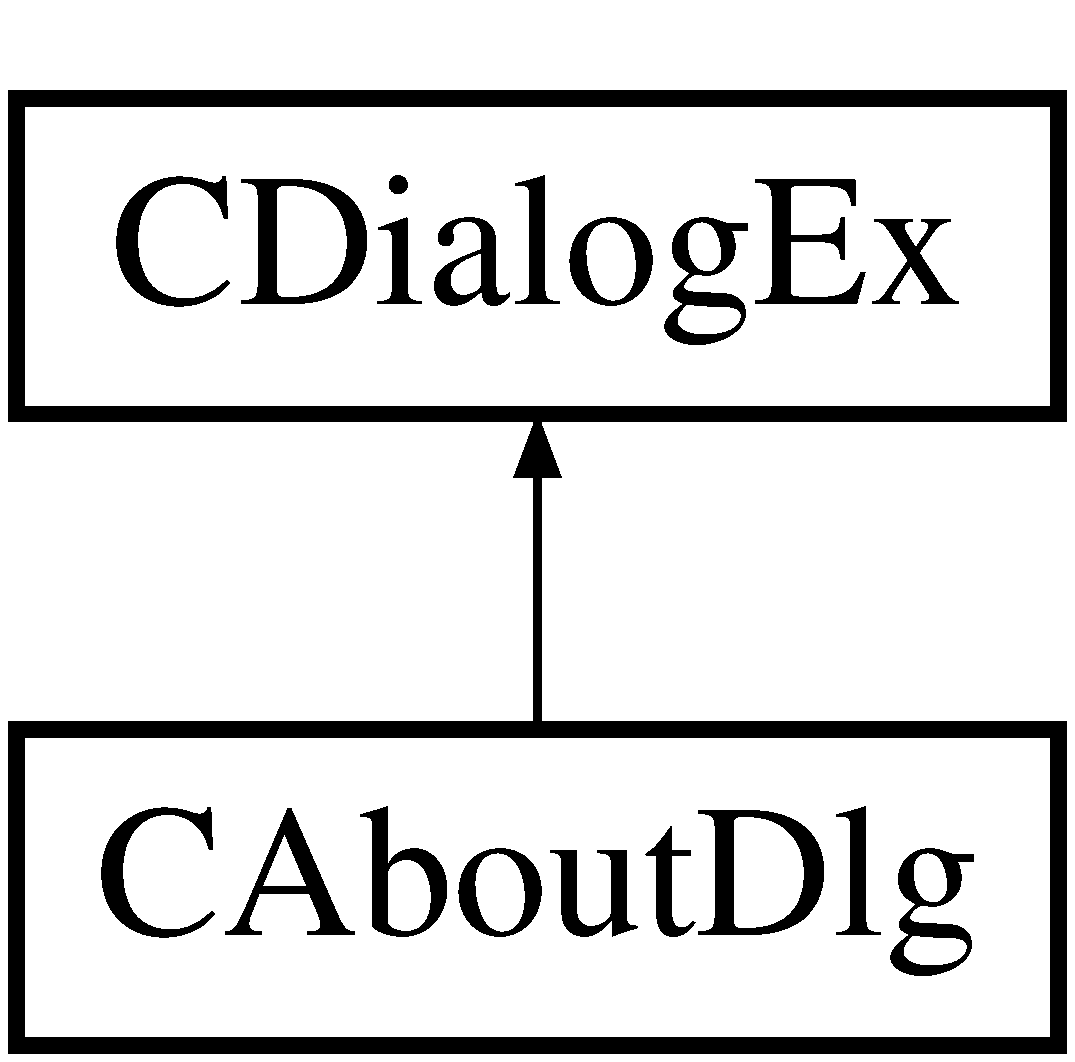
\includegraphics[height=2.000000cm]{class_c_about_dlg}
\end{center}
\end{figure}
\subsection*{Protected Member Functions}
\begin{DoxyCompactItemize}
\item 
\mbox{\Hypertarget{class_c_about_dlg_ab83db7484fec957282d7d5a21aed4df4}\label{class_c_about_dlg_ab83db7484fec957282d7d5a21aed4df4}} 
virtual void {\bfseries Do\+Data\+Exchange} (C\+Data\+Exchange $\ast$p\+DX)
\end{DoxyCompactItemize}


The documentation for this class was generated from the following file\+:\begin{DoxyCompactItemize}
\item 
Step2.\+cpp\end{DoxyCompactItemize}

\hypertarget{class_c_aquarium}{}\section{C\+Aquarium Class Reference}
\label{class_c_aquarium}\index{C\+Aquarium@{C\+Aquarium}}


{\ttfamily \#include $<$Aquarium.\+h$>$}

\subsection*{Public Member Functions}
\begin{DoxyCompactItemize}
\item 
\mbox{\hyperlink{class_c_aquarium_ab6ba8b1abd87437ff66748e82173a5a8}{C\+Aquarium}} ()
\item 
virtual \mbox{\hyperlink{class_c_aquarium_ab1baf78dc047af2b8cab8982e1446875}{$\sim$\+C\+Aquarium}} ()
\item 
void \mbox{\hyperlink{class_c_aquarium_a20b4899158d1ba4bc41217630d47e180}{On\+Draw}} (Gdiplus\+::\+Graphics $\ast$graphics)
\item 
void \mbox{\hyperlink{class_c_aquarium_a85063d05c147cf80f54182016fe12d64}{Add}} (std\+::shared\+\_\+ptr$<$ \mbox{\hyperlink{class_c_item}{C\+Item}} $>$ item)
\item 
std\+::shared\+\_\+ptr$<$ \mbox{\hyperlink{class_c_item}{C\+Item}} $>$ \mbox{\hyperlink{class_c_aquarium_a7129486467e76938fbc049723f9187f3}{Hit\+Test}} (int x, int y)
\item 
void \mbox{\hyperlink{class_c_aquarium_a2ee2a7d57d9f5d9996f9f9b468c98a2b}{Push\+To\+Front}} (std\+::shared\+\_\+ptr$<$ \mbox{\hyperlink{class_c_item}{C\+Item}} $>$ item)
\item 
bool \mbox{\hyperlink{class_c_aquarium_a111b3c61aa0cd3f8bdda1e2bc6b63ed1}{Killing}} (\mbox{\hyperlink{class_c_item}{C\+Item}} $\ast$item)
\item 
void \mbox{\hyperlink{class_c_aquarium_adc9e22446b161ec23acdef368cb8ac2e}{Clear}} ()
\item 
void \mbox{\hyperlink{class_c_aquarium_acace2b3a8c1ed29011d83ac8231c66d0}{Save}} (const std\+::wstring \&filename)
\item 
void \mbox{\hyperlink{class_c_aquarium_aeffc772356405adc8b79beba77c25d0f}{Update}} (double elapsed)
\item 
void \mbox{\hyperlink{class_c_aquarium_a21faac4da17cea923d8f7a5cebe45141}{Load}} (const std\+::wstring \&filename)
\item 
int \mbox{\hyperlink{class_c_aquarium_a002b101c76d468db423da85b9eb56210}{Get\+Width}} () const
\item 
int \mbox{\hyperlink{class_c_aquarium_a6553dfa3238a4e731dbdbe0ccd6ce956}{Get\+Height}} () const
\end{DoxyCompactItemize}


\subsection{Detailed Description}
Represents an aquarium 

\subsection{Constructor \& Destructor Documentation}
\mbox{\Hypertarget{class_c_aquarium_ab6ba8b1abd87437ff66748e82173a5a8}\label{class_c_aquarium_ab6ba8b1abd87437ff66748e82173a5a8}} 
\index{C\+Aquarium@{C\+Aquarium}!C\+Aquarium@{C\+Aquarium}}
\index{C\+Aquarium@{C\+Aquarium}!C\+Aquarium@{C\+Aquarium}}
\subsubsection{\texorpdfstring{C\+Aquarium()}{CAquarium()}}
{\footnotesize\ttfamily C\+Aquarium\+::\+C\+Aquarium (\begin{DoxyParamCaption}{ }\end{DoxyParamCaption})}

Constructor \mbox{\Hypertarget{class_c_aquarium_ab1baf78dc047af2b8cab8982e1446875}\label{class_c_aquarium_ab1baf78dc047af2b8cab8982e1446875}} 
\index{C\+Aquarium@{C\+Aquarium}!````~C\+Aquarium@{$\sim$\+C\+Aquarium}}
\index{````~C\+Aquarium@{$\sim$\+C\+Aquarium}!C\+Aquarium@{C\+Aquarium}}
\subsubsection{\texorpdfstring{$\sim$\+C\+Aquarium()}{~CAquarium()}}
{\footnotesize\ttfamily C\+Aquarium\+::$\sim$\+C\+Aquarium (\begin{DoxyParamCaption}{ }\end{DoxyParamCaption})\hspace{0.3cm}{\ttfamily [virtual]}}

Destructor 

\subsection{Member Function Documentation}
\mbox{\Hypertarget{class_c_aquarium_a85063d05c147cf80f54182016fe12d64}\label{class_c_aquarium_a85063d05c147cf80f54182016fe12d64}} 
\index{C\+Aquarium@{C\+Aquarium}!Add@{Add}}
\index{Add@{Add}!C\+Aquarium@{C\+Aquarium}}
\subsubsection{\texorpdfstring{Add()}{Add()}}
{\footnotesize\ttfamily void C\+Aquarium\+::\+Add (\begin{DoxyParamCaption}\item[{std\+::shared\+\_\+ptr$<$ \mbox{\hyperlink{class_c_item}{C\+Item}} $>$}]{item }\end{DoxyParamCaption})}

Add an item to the aquarium 
\begin{DoxyParams}{Parameters}
{\em item} & New item to add \\
\hline
\end{DoxyParams}
\mbox{\Hypertarget{class_c_aquarium_adc9e22446b161ec23acdef368cb8ac2e}\label{class_c_aquarium_adc9e22446b161ec23acdef368cb8ac2e}} 
\index{C\+Aquarium@{C\+Aquarium}!Clear@{Clear}}
\index{Clear@{Clear}!C\+Aquarium@{C\+Aquarium}}
\subsubsection{\texorpdfstring{Clear()}{Clear()}}
{\footnotesize\ttfamily void C\+Aquarium\+::\+Clear (\begin{DoxyParamCaption}{ }\end{DoxyParamCaption})}

Clear the aquarium data.

Deletes all known items in the aquarium. \mbox{\Hypertarget{class_c_aquarium_a6553dfa3238a4e731dbdbe0ccd6ce956}\label{class_c_aquarium_a6553dfa3238a4e731dbdbe0ccd6ce956}} 
\index{C\+Aquarium@{C\+Aquarium}!Get\+Height@{Get\+Height}}
\index{Get\+Height@{Get\+Height}!C\+Aquarium@{C\+Aquarium}}
\subsubsection{\texorpdfstring{Get\+Height()}{GetHeight()}}
{\footnotesize\ttfamily int C\+Aquarium\+::\+Get\+Height (\begin{DoxyParamCaption}{ }\end{DoxyParamCaption}) const\hspace{0.3cm}{\ttfamily [inline]}}

Get the height of the aquarium \begin{DoxyReturn}{Returns}
Aquarium height 
\end{DoxyReturn}
\mbox{\Hypertarget{class_c_aquarium_a002b101c76d468db423da85b9eb56210}\label{class_c_aquarium_a002b101c76d468db423da85b9eb56210}} 
\index{C\+Aquarium@{C\+Aquarium}!Get\+Width@{Get\+Width}}
\index{Get\+Width@{Get\+Width}!C\+Aquarium@{C\+Aquarium}}
\subsubsection{\texorpdfstring{Get\+Width()}{GetWidth()}}
{\footnotesize\ttfamily int C\+Aquarium\+::\+Get\+Width (\begin{DoxyParamCaption}{ }\end{DoxyParamCaption}) const\hspace{0.3cm}{\ttfamily [inline]}}

Get the width of the aquarium \begin{DoxyReturn}{Returns}
Aquarium width 
\end{DoxyReturn}
\mbox{\Hypertarget{class_c_aquarium_a7129486467e76938fbc049723f9187f3}\label{class_c_aquarium_a7129486467e76938fbc049723f9187f3}} 
\index{C\+Aquarium@{C\+Aquarium}!Hit\+Test@{Hit\+Test}}
\index{Hit\+Test@{Hit\+Test}!C\+Aquarium@{C\+Aquarium}}
\subsubsection{\texorpdfstring{Hit\+Test()}{HitTest()}}
{\footnotesize\ttfamily std\+::shared\+\_\+ptr$<$ \mbox{\hyperlink{class_c_item}{C\+Item}} $>$ C\+Aquarium\+::\+Hit\+Test (\begin{DoxyParamCaption}\item[{int}]{x,  }\item[{int}]{y }\end{DoxyParamCaption})}

Test an x,y click location to see if it clicked on some item in the aquarium. 
\begin{DoxyParams}{Parameters}
{\em x} & X location \\
\hline
{\em y} & Y location \\
\hline
\end{DoxyParams}
\begin{DoxyReturn}{Returns}
Pointer to item we clicked on or nullptr if none. 
\end{DoxyReturn}
\mbox{\Hypertarget{class_c_aquarium_a111b3c61aa0cd3f8bdda1e2bc6b63ed1}\label{class_c_aquarium_a111b3c61aa0cd3f8bdda1e2bc6b63ed1}} 
\index{C\+Aquarium@{C\+Aquarium}!Killing@{Killing}}
\index{Killing@{Killing}!C\+Aquarium@{C\+Aquarium}}
\subsubsection{\texorpdfstring{Killing()}{Killing()}}
{\footnotesize\ttfamily bool C\+Aquarium\+::\+Killing (\begin{DoxyParamCaption}\item[{\mbox{\hyperlink{class_c_item}{C\+Item}} $\ast$}]{eater }\end{DoxyParamCaption})}

We are passed a pointer to a fish that eats. We check to see if there are any fish it is currently over. If so, eat them! 
\begin{DoxyParams}{Parameters}
{\em item} & Item we are testing \\
\hline
{\em eater} & is the karp \\
\hline
\end{DoxyParams}
\begin{DoxyReturn}{Returns}
true if a fish is eaten 
\end{DoxyReturn}
\mbox{\Hypertarget{class_c_aquarium_a21faac4da17cea923d8f7a5cebe45141}\label{class_c_aquarium_a21faac4da17cea923d8f7a5cebe45141}} 
\index{C\+Aquarium@{C\+Aquarium}!Load@{Load}}
\index{Load@{Load}!C\+Aquarium@{C\+Aquarium}}
\subsubsection{\texorpdfstring{Load()}{Load()}}
{\footnotesize\ttfamily void C\+Aquarium\+::\+Load (\begin{DoxyParamCaption}\item[{const std\+::wstring \&}]{filename }\end{DoxyParamCaption})}

Load the aquarium from a .aqua X\+ML file.

Opens the X\+ML file and reads the nodes, creating items as appropriate.


\begin{DoxyParams}{Parameters}
{\em filename} & The filename of the file to load the aquarium from. \\
\hline
\end{DoxyParams}
\mbox{\Hypertarget{class_c_aquarium_a20b4899158d1ba4bc41217630d47e180}\label{class_c_aquarium_a20b4899158d1ba4bc41217630d47e180}} 
\index{C\+Aquarium@{C\+Aquarium}!On\+Draw@{On\+Draw}}
\index{On\+Draw@{On\+Draw}!C\+Aquarium@{C\+Aquarium}}
\subsubsection{\texorpdfstring{On\+Draw()}{OnDraw()}}
{\footnotesize\ttfamily void C\+Aquarium\+::\+On\+Draw (\begin{DoxyParamCaption}\item[{Gdiplus\+::\+Graphics $\ast$}]{graphics }\end{DoxyParamCaption})}

Draw the aquarium 
\begin{DoxyParams}{Parameters}
{\em graphics} & The G\+D\+I+ graphics context to draw on \\
\hline
\end{DoxyParams}
\mbox{\Hypertarget{class_c_aquarium_a2ee2a7d57d9f5d9996f9f9b468c98a2b}\label{class_c_aquarium_a2ee2a7d57d9f5d9996f9f9b468c98a2b}} 
\index{C\+Aquarium@{C\+Aquarium}!Push\+To\+Front@{Push\+To\+Front}}
\index{Push\+To\+Front@{Push\+To\+Front}!C\+Aquarium@{C\+Aquarium}}
\subsubsection{\texorpdfstring{Push\+To\+Front()}{PushToFront()}}
{\footnotesize\ttfamily void C\+Aquarium\+::\+Push\+To\+Front (\begin{DoxyParamCaption}\item[{std\+::shared\+\_\+ptr$<$ \mbox{\hyperlink{class_c_item}{C\+Item}} $>$}]{item }\end{DoxyParamCaption})}

Function to push to front of list 
\begin{DoxyParams}{Parameters}
{\em item} & \\
\hline
\end{DoxyParams}
\mbox{\Hypertarget{class_c_aquarium_acace2b3a8c1ed29011d83ac8231c66d0}\label{class_c_aquarium_acace2b3a8c1ed29011d83ac8231c66d0}} 
\index{C\+Aquarium@{C\+Aquarium}!Save@{Save}}
\index{Save@{Save}!C\+Aquarium@{C\+Aquarium}}
\subsubsection{\texorpdfstring{Save()}{Save()}}
{\footnotesize\ttfamily void C\+Aquarium\+::\+Save (\begin{DoxyParamCaption}\item[{const std\+::wstring \&}]{filename }\end{DoxyParamCaption})}

Save the aquarium as a .aqua X\+ML file.

Open an X\+ML file and stream the aquarium data to it.


\begin{DoxyParams}{Parameters}
{\em filename} & The filename of the file to save the aquarium to \\
\hline
\end{DoxyParams}
\mbox{\Hypertarget{class_c_aquarium_aeffc772356405adc8b79beba77c25d0f}\label{class_c_aquarium_aeffc772356405adc8b79beba77c25d0f}} 
\index{C\+Aquarium@{C\+Aquarium}!Update@{Update}}
\index{Update@{Update}!C\+Aquarium@{C\+Aquarium}}
\subsubsection{\texorpdfstring{Update()}{Update()}}
{\footnotesize\ttfamily void C\+Aquarium\+::\+Update (\begin{DoxyParamCaption}\item[{double}]{elapsed }\end{DoxyParamCaption})}

Handle updates for animation 
\begin{DoxyParams}{Parameters}
{\em elapsed} & The time since the last update \\
\hline
\end{DoxyParams}


The documentation for this class was generated from the following files\+:\begin{DoxyCompactItemize}
\item 
\mbox{\hyperlink{_aquarium_8h}{Aquarium.\+h}}\item 
\mbox{\hyperlink{_aquarium_8cpp}{Aquarium.\+cpp}}\end{DoxyCompactItemize}

\hypertarget{class_c_child_view}{}\section{C\+Child\+View Class Reference}
\label{class_c_child_view}\index{C\+Child\+View@{C\+Child\+View}}


{\ttfamily \#include $<$Child\+View.\+h$>$}

Inheritance diagram for C\+Child\+View\+:\begin{figure}[H]
\begin{center}
\leavevmode
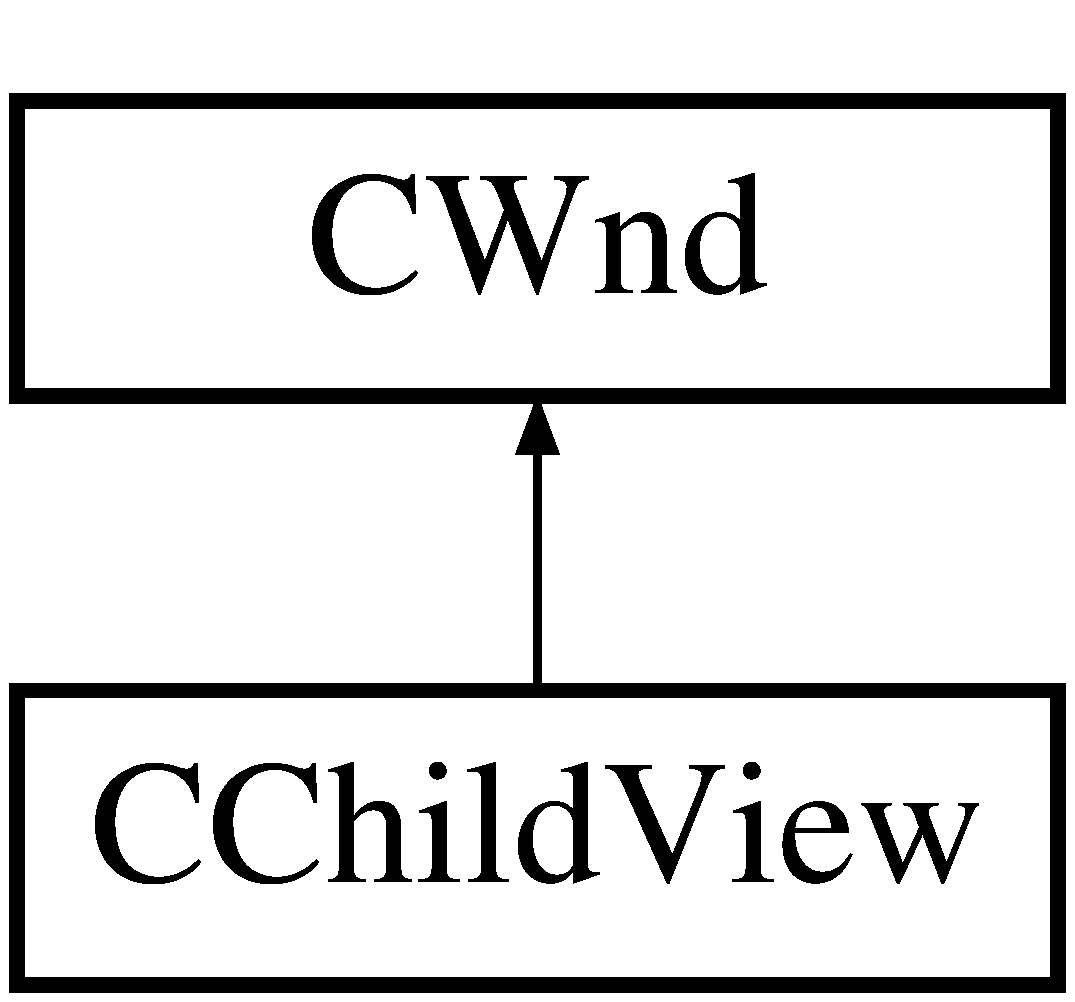
\includegraphics[height=2.000000cm]{class_c_child_view}
\end{center}
\end{figure}
\subsection*{Public Member Functions}
\begin{DoxyCompactItemize}
\item 
\mbox{\hyperlink{class_c_child_view_aff5af7c162c10755edbe58f260ded6d4}{C\+Child\+View}} ()
\item 
virtual \mbox{\hyperlink{class_c_child_view_a5b033b5e0a130950719a173b86418698}{$\sim$\+C\+Child\+View}} ()
\item 
afx\+\_\+msg void \mbox{\hyperlink{class_c_child_view_ad05faefbdb17d1c73f85de75b01a1ac1}{On\+Addfish\+Betafish}} ()
\item 
afx\+\_\+msg void \mbox{\hyperlink{class_c_child_view_ad3cb2f8d9fa9a6fb06989513dee5a8bc}{On\+Mouse\+Move}} (U\+I\+NT n\+Flags, C\+Point point)
\item 
afx\+\_\+msg void \mbox{\hyperlink{class_c_child_view_af513a57c45ce8b9dcc09dd934e228534}{On\+L\+Button\+Down}} (U\+I\+NT n\+Flags, C\+Point point)
\item 
afx\+\_\+msg void \mbox{\hyperlink{class_c_child_view_ae81948a77ebf3744bd0f9449af57ee21}{On\+L\+Button\+Up}} (U\+I\+NT n\+Flags, C\+Point point)
\item 
afx\+\_\+msg B\+O\+OL \mbox{\hyperlink{class_c_child_view_a6060e6d09d522d345dcee5a01d41c1f0}{On\+Erase\+Bkgnd}} (C\+DC $\ast$p\+DC)
\item 
afx\+\_\+msg void \mbox{\hyperlink{class_c_child_view_acb27b77bb4d6f4997c7d2d94f1a4e14c}{On\+Addfish\+Doryfish}} ()
\item 
afx\+\_\+msg void \mbox{\hyperlink{class_c_child_view_a6fddae71d821dd64cfae1359e8a33a62}{On\+Addfish\+Nemofish}} ()
\item 
afx\+\_\+msg void \mbox{\hyperlink{class_c_child_view_a0d3175bb87c2e24572d6c0364abebd07}{On\+Addfish\+Killerkarp}} ()
\item 
afx\+\_\+msg void \mbox{\hyperlink{class_c_child_view_aaf8f6acf9df7bdfa17f9dfcfa60d7883}{On\+Adddecor\+Decorcastle}} ()
\item 
afx\+\_\+msg void \mbox{\hyperlink{class_c_child_view_a2f79325c40f3a93227e60498b2135785}{On\+File\+Saveas}} ()
\item 
afx\+\_\+msg void \mbox{\hyperlink{class_c_child_view_a6e69d915eea1631da5f8a8d8d5a2c101}{On\+File\+Open32780}} ()
\item 
\mbox{\Hypertarget{class_c_child_view_a4c6bb8bd631cee84bb80c948f3d6d98a}\label{class_c_child_view_a4c6bb8bd631cee84bb80c948f3d6d98a}} 
afx\+\_\+msg void {\bfseries On\+Timer} (U\+I\+N\+T\+\_\+\+P\+TR n\+I\+D\+Event)
\end{DoxyCompactItemize}
\subsection*{Protected Member Functions}
\begin{DoxyCompactItemize}
\item 
afx\+\_\+msg void \mbox{\hyperlink{class_c_child_view_a8ea6d42631a4f9f446923ff864b239ab}{On\+Paint}} ()
\item 
\mbox{\Hypertarget{class_c_child_view_a072cbcba60255377ac9d82aed9a14ce8}\label{class_c_child_view_a072cbcba60255377ac9d82aed9a14ce8}} 
virtual B\+O\+OL {\bfseries Pre\+Create\+Window} (C\+R\+E\+A\+T\+E\+S\+T\+R\+U\+CT \&cs)
\end{DoxyCompactItemize}


\subsection{Detailed Description}
The child window our program draws in. 

\subsection{Constructor \& Destructor Documentation}
\mbox{\Hypertarget{class_c_child_view_aff5af7c162c10755edbe58f260ded6d4}\label{class_c_child_view_aff5af7c162c10755edbe58f260ded6d4}} 
\index{C\+Child\+View@{C\+Child\+View}!C\+Child\+View@{C\+Child\+View}}
\index{C\+Child\+View@{C\+Child\+View}!C\+Child\+View@{C\+Child\+View}}
\subsubsection{\texorpdfstring{C\+Child\+View()}{CChildView()}}
{\footnotesize\ttfamily C\+Child\+View\+::\+C\+Child\+View (\begin{DoxyParamCaption}{ }\end{DoxyParamCaption})}

Constructor \mbox{\Hypertarget{class_c_child_view_a5b033b5e0a130950719a173b86418698}\label{class_c_child_view_a5b033b5e0a130950719a173b86418698}} 
\index{C\+Child\+View@{C\+Child\+View}!````~C\+Child\+View@{$\sim$\+C\+Child\+View}}
\index{````~C\+Child\+View@{$\sim$\+C\+Child\+View}!C\+Child\+View@{C\+Child\+View}}
\subsubsection{\texorpdfstring{$\sim$\+C\+Child\+View()}{~CChildView()}}
{\footnotesize\ttfamily C\+Child\+View\+::$\sim$\+C\+Child\+View (\begin{DoxyParamCaption}{ }\end{DoxyParamCaption})\hspace{0.3cm}{\ttfamily [virtual]}}

Destructor 

\subsection{Member Function Documentation}
\mbox{\Hypertarget{class_c_child_view_aaf8f6acf9df7bdfa17f9dfcfa60d7883}\label{class_c_child_view_aaf8f6acf9df7bdfa17f9dfcfa60d7883}} 
\index{C\+Child\+View@{C\+Child\+View}!On\+Adddecor\+Decorcastle@{On\+Adddecor\+Decorcastle}}
\index{On\+Adddecor\+Decorcastle@{On\+Adddecor\+Decorcastle}!C\+Child\+View@{C\+Child\+View}}
\subsubsection{\texorpdfstring{On\+Adddecor\+Decorcastle()}{OnAdddecorDecorcastle()}}
{\footnotesize\ttfamily void C\+Child\+View\+::\+On\+Adddecor\+Decorcastle (\begin{DoxyParamCaption}{ }\end{DoxyParamCaption})}

Castle event handler for menu option. \mbox{\Hypertarget{class_c_child_view_ad05faefbdb17d1c73f85de75b01a1ac1}\label{class_c_child_view_ad05faefbdb17d1c73f85de75b01a1ac1}} 
\index{C\+Child\+View@{C\+Child\+View}!On\+Addfish\+Betafish@{On\+Addfish\+Betafish}}
\index{On\+Addfish\+Betafish@{On\+Addfish\+Betafish}!C\+Child\+View@{C\+Child\+View}}
\subsubsection{\texorpdfstring{On\+Addfish\+Betafish()}{OnAddfishBetafish()}}
{\footnotesize\ttfamily void C\+Child\+View\+::\+On\+Addfish\+Betafish (\begin{DoxyParamCaption}{ }\end{DoxyParamCaption})}

Function to add on a Beta Fish \mbox{\Hypertarget{class_c_child_view_acb27b77bb4d6f4997c7d2d94f1a4e14c}\label{class_c_child_view_acb27b77bb4d6f4997c7d2d94f1a4e14c}} 
\index{C\+Child\+View@{C\+Child\+View}!On\+Addfish\+Doryfish@{On\+Addfish\+Doryfish}}
\index{On\+Addfish\+Doryfish@{On\+Addfish\+Doryfish}!C\+Child\+View@{C\+Child\+View}}
\subsubsection{\texorpdfstring{On\+Addfish\+Doryfish()}{OnAddfishDoryfish()}}
{\footnotesize\ttfamily void C\+Child\+View\+::\+On\+Addfish\+Doryfish (\begin{DoxyParamCaption}{ }\end{DoxyParamCaption})}

Fish\+Dory event handler for menu option. \mbox{\Hypertarget{class_c_child_view_a0d3175bb87c2e24572d6c0364abebd07}\label{class_c_child_view_a0d3175bb87c2e24572d6c0364abebd07}} 
\index{C\+Child\+View@{C\+Child\+View}!On\+Addfish\+Killerkarp@{On\+Addfish\+Killerkarp}}
\index{On\+Addfish\+Killerkarp@{On\+Addfish\+Killerkarp}!C\+Child\+View@{C\+Child\+View}}
\subsubsection{\texorpdfstring{On\+Addfish\+Killerkarp()}{OnAddfishKillerkarp()}}
{\footnotesize\ttfamily void C\+Child\+View\+::\+On\+Addfish\+Killerkarp (\begin{DoxyParamCaption}{ }\end{DoxyParamCaption})}

Carp event handler for menu option. \mbox{\Hypertarget{class_c_child_view_a6fddae71d821dd64cfae1359e8a33a62}\label{class_c_child_view_a6fddae71d821dd64cfae1359e8a33a62}} 
\index{C\+Child\+View@{C\+Child\+View}!On\+Addfish\+Nemofish@{On\+Addfish\+Nemofish}}
\index{On\+Addfish\+Nemofish@{On\+Addfish\+Nemofish}!C\+Child\+View@{C\+Child\+View}}
\subsubsection{\texorpdfstring{On\+Addfish\+Nemofish()}{OnAddfishNemofish()}}
{\footnotesize\ttfamily void C\+Child\+View\+::\+On\+Addfish\+Nemofish (\begin{DoxyParamCaption}{ }\end{DoxyParamCaption})}

Fish\+Nemo event handler for menu option. \mbox{\Hypertarget{class_c_child_view_a6060e6d09d522d345dcee5a01d41c1f0}\label{class_c_child_view_a6060e6d09d522d345dcee5a01d41c1f0}} 
\index{C\+Child\+View@{C\+Child\+View}!On\+Erase\+Bkgnd@{On\+Erase\+Bkgnd}}
\index{On\+Erase\+Bkgnd@{On\+Erase\+Bkgnd}!C\+Child\+View@{C\+Child\+View}}
\subsubsection{\texorpdfstring{On\+Erase\+Bkgnd()}{OnEraseBkgnd()}}
{\footnotesize\ttfamily B\+O\+OL C\+Child\+View\+::\+On\+Erase\+Bkgnd (\begin{DoxyParamCaption}\item[{C\+DC $\ast$}]{p\+DC }\end{DoxyParamCaption})}

Erase the background

This is disabled to eliminate flicker 
\begin{DoxyParams}{Parameters}
{\em p\+DC} & Device context \\
\hline
\end{DoxyParams}
\begin{DoxyReturn}{Returns}
F\+A\+L\+SE 
\end{DoxyReturn}
\mbox{\Hypertarget{class_c_child_view_a6e69d915eea1631da5f8a8d8d5a2c101}\label{class_c_child_view_a6e69d915eea1631da5f8a8d8d5a2c101}} 
\index{C\+Child\+View@{C\+Child\+View}!On\+File\+Open32780@{On\+File\+Open32780}}
\index{On\+File\+Open32780@{On\+File\+Open32780}!C\+Child\+View@{C\+Child\+View}}
\subsubsection{\texorpdfstring{On\+File\+Open32780()}{OnFileOpen32780()}}
{\footnotesize\ttfamily void C\+Child\+View\+::\+On\+File\+Open32780 (\begin{DoxyParamCaption}{ }\end{DoxyParamCaption})}

This function is called when an File Open menu item is selected.

It loads the aquarium from a file. \mbox{\Hypertarget{class_c_child_view_a2f79325c40f3a93227e60498b2135785}\label{class_c_child_view_a2f79325c40f3a93227e60498b2135785}} 
\index{C\+Child\+View@{C\+Child\+View}!On\+File\+Saveas@{On\+File\+Saveas}}
\index{On\+File\+Saveas@{On\+File\+Saveas}!C\+Child\+View@{C\+Child\+View}}
\subsubsection{\texorpdfstring{On\+File\+Saveas()}{OnFileSaveas()}}
{\footnotesize\ttfamily void C\+Child\+View\+::\+On\+File\+Saveas (\begin{DoxyParamCaption}{ }\end{DoxyParamCaption})}

This function is called when an File Saveas menu item is selected.

It saves the aquarium as an X\+ML file. \mbox{\Hypertarget{class_c_child_view_af513a57c45ce8b9dcc09dd934e228534}\label{class_c_child_view_af513a57c45ce8b9dcc09dd934e228534}} 
\index{C\+Child\+View@{C\+Child\+View}!On\+L\+Button\+Down@{On\+L\+Button\+Down}}
\index{On\+L\+Button\+Down@{On\+L\+Button\+Down}!C\+Child\+View@{C\+Child\+View}}
\subsubsection{\texorpdfstring{On\+L\+Button\+Down()}{OnLButtonDown()}}
{\footnotesize\ttfamily void C\+Child\+View\+::\+On\+L\+Button\+Down (\begin{DoxyParamCaption}\item[{U\+I\+NT}]{n\+Flags,  }\item[{C\+Point}]{point }\end{DoxyParamCaption})}

Called when there is a left mouse button press 
\begin{DoxyParams}{Parameters}
{\em n\+Flags} & Flags associated with the mouse button press \\
\hline
{\em point} & Where the button was pressed \\
\hline
\end{DoxyParams}
\mbox{\Hypertarget{class_c_child_view_ae81948a77ebf3744bd0f9449af57ee21}\label{class_c_child_view_ae81948a77ebf3744bd0f9449af57ee21}} 
\index{C\+Child\+View@{C\+Child\+View}!On\+L\+Button\+Up@{On\+L\+Button\+Up}}
\index{On\+L\+Button\+Up@{On\+L\+Button\+Up}!C\+Child\+View@{C\+Child\+View}}
\subsubsection{\texorpdfstring{On\+L\+Button\+Up()}{OnLButtonUp()}}
{\footnotesize\ttfamily void C\+Child\+View\+::\+On\+L\+Button\+Up (\begin{DoxyParamCaption}\item[{U\+I\+NT}]{n\+Flags,  }\item[{C\+Point}]{point }\end{DoxyParamCaption})}

Called when the left mouse button is released 
\begin{DoxyParams}{Parameters}
{\em n\+Flags} & Flags associated with the mouse button release \\
\hline
{\em point} & Where the button was pressed \\
\hline
\end{DoxyParams}
\mbox{\Hypertarget{class_c_child_view_ad3cb2f8d9fa9a6fb06989513dee5a8bc}\label{class_c_child_view_ad3cb2f8d9fa9a6fb06989513dee5a8bc}} 
\index{C\+Child\+View@{C\+Child\+View}!On\+Mouse\+Move@{On\+Mouse\+Move}}
\index{On\+Mouse\+Move@{On\+Mouse\+Move}!C\+Child\+View@{C\+Child\+View}}
\subsubsection{\texorpdfstring{On\+Mouse\+Move()}{OnMouseMove()}}
{\footnotesize\ttfamily void C\+Child\+View\+::\+On\+Mouse\+Move (\begin{DoxyParamCaption}\item[{U\+I\+NT}]{n\+Flags,  }\item[{C\+Point}]{point }\end{DoxyParamCaption})}

Called when the mouse is moved 
\begin{DoxyParams}{Parameters}
{\em n\+Flags} & Flags associated with the mouse movement \\
\hline
{\em point} & Where the button was pressed \\
\hline
\end{DoxyParams}
\mbox{\Hypertarget{class_c_child_view_a8ea6d42631a4f9f446923ff864b239ab}\label{class_c_child_view_a8ea6d42631a4f9f446923ff864b239ab}} 
\index{C\+Child\+View@{C\+Child\+View}!On\+Paint@{On\+Paint}}
\index{On\+Paint@{On\+Paint}!C\+Child\+View@{C\+Child\+View}}
\subsubsection{\texorpdfstring{On\+Paint()}{OnPaint()}}
{\footnotesize\ttfamily void C\+Child\+View\+::\+On\+Paint (\begin{DoxyParamCaption}{ }\end{DoxyParamCaption})\hspace{0.3cm}{\ttfamily [protected]}}

This function is called to draw in the window.

This function is called in response to a drawing message whenever we need to redraw the window on the screen. It is responsible for painting the window. 

The documentation for this class was generated from the following files\+:\begin{DoxyCompactItemize}
\item 
\mbox{\hyperlink{_child_view_8h}{Child\+View.\+h}}\item 
\mbox{\hyperlink{_child_view_8cpp}{Child\+View.\+cpp}}\end{DoxyCompactItemize}

\hypertarget{class_c_fish_beta}{}\section{C\+Fish\+Beta Class Reference}
\label{class_c_fish_beta}\index{C\+Fish\+Beta@{C\+Fish\+Beta}}


{\ttfamily \#include $<$Fish\+Beta.\+h$>$}

Inheritance diagram for C\+Fish\+Beta\+:\begin{figure}[H]
\begin{center}
\leavevmode
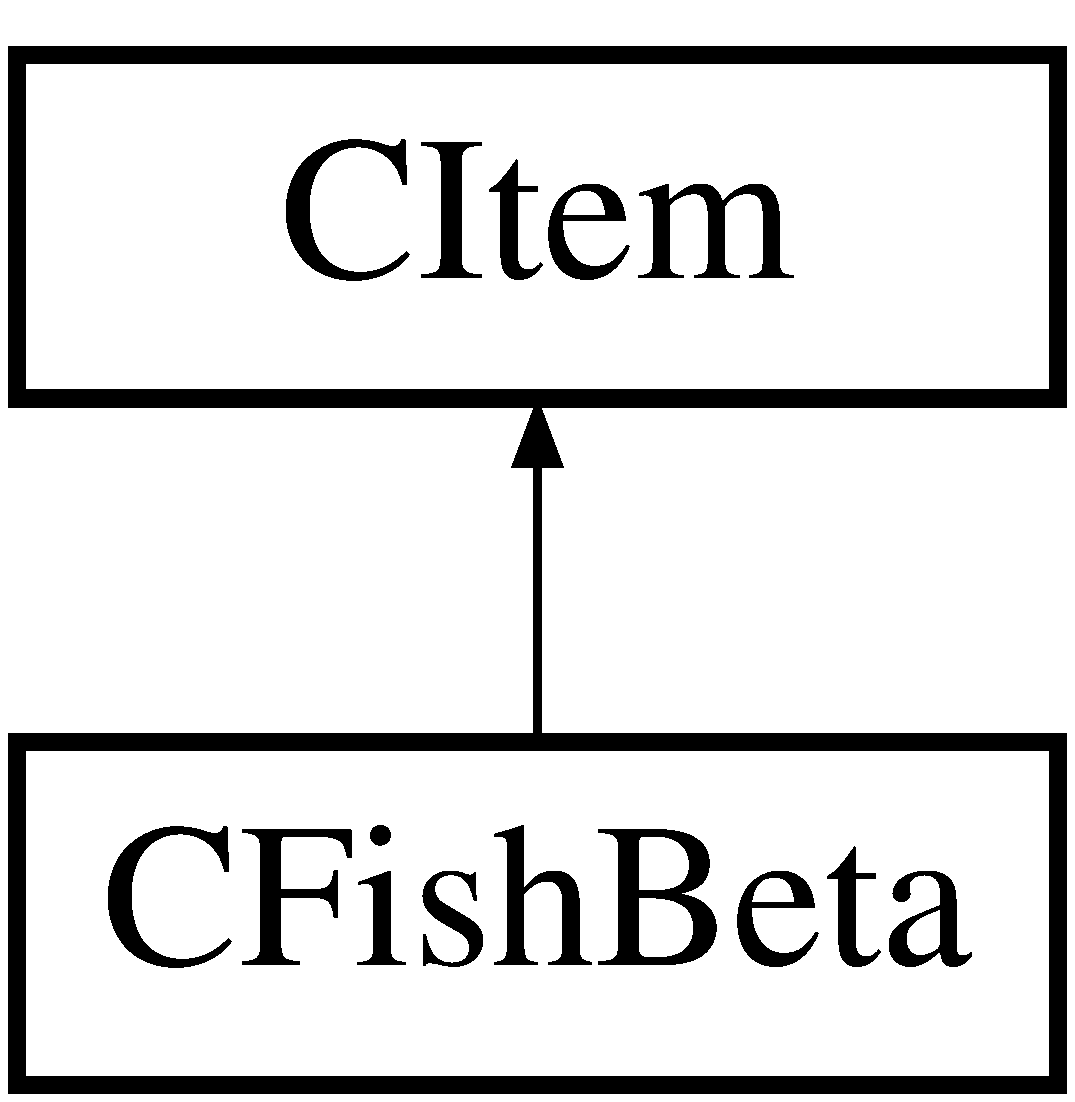
\includegraphics[height=3.000000cm]{class_c_fish_beta}
\end{center}
\end{figure}
\subsection*{Public Member Functions}
\begin{DoxyCompactItemize}
\item 
\mbox{\hyperlink{class_c_fish_beta_a021073e2e0034271cd7e776b1e3fed29}{C\+Fish\+Beta}} (\mbox{\hyperlink{class_c_aquarium}{C\+Aquarium}} $\ast$aquarium)
\item 
\mbox{\Hypertarget{class_c_fish_beta_a4e4d132618735adad44d04c9c40687ca}\label{class_c_fish_beta_a4e4d132618735adad44d04c9c40687ca}} 
\mbox{\hyperlink{class_c_fish_beta_a4e4d132618735adad44d04c9c40687ca}{C\+Fish\+Beta}} ()=delete
\begin{DoxyCompactList}\small\item\em Default constructor (disabled) \end{DoxyCompactList}\item 
\mbox{\Hypertarget{class_c_fish_beta_adbf3559baac135dff393729c51b1ab31}\label{class_c_fish_beta_adbf3559baac135dff393729c51b1ab31}} 
\mbox{\hyperlink{class_c_fish_beta_adbf3559baac135dff393729c51b1ab31}{C\+Fish\+Beta}} (const \mbox{\hyperlink{class_c_fish_beta}{C\+Fish\+Beta}} \&)=delete
\begin{DoxyCompactList}\small\item\em Copy constructor (disabled) \end{DoxyCompactList}\item 
virtual std\+::shared\+\_\+ptr$<$ \mbox{\hyperlink{classxmlnode_1_1_c_xml_node}{xmlnode\+::\+C\+Xml\+Node}} $>$ \mbox{\hyperlink{class_c_fish_beta_a0be2886a531ede77bfa5338fec71d71b}{Xml\+Save}} (const std\+::shared\+\_\+ptr$<$ \mbox{\hyperlink{classxmlnode_1_1_c_xml_node}{xmlnode\+::\+C\+Xml\+Node}} $>$ \&node) override
\item 
\mbox{\hyperlink{class_c_fish_beta_abd932894ad25a70f03c79c4f0f00fff4}{$\sim$\+C\+Fish\+Beta}} ()
\end{DoxyCompactItemize}
\subsection*{Additional Inherited Members}


\subsection{Detailed Description}
Implements a Beta fish 

\subsection{Constructor \& Destructor Documentation}
\mbox{\Hypertarget{class_c_fish_beta_a021073e2e0034271cd7e776b1e3fed29}\label{class_c_fish_beta_a021073e2e0034271cd7e776b1e3fed29}} 
\index{C\+Fish\+Beta@{C\+Fish\+Beta}!C\+Fish\+Beta@{C\+Fish\+Beta}}
\index{C\+Fish\+Beta@{C\+Fish\+Beta}!C\+Fish\+Beta@{C\+Fish\+Beta}}
\subsubsection{\texorpdfstring{C\+Fish\+Beta()}{CFishBeta()}}
{\footnotesize\ttfamily C\+Fish\+Beta\+::\+C\+Fish\+Beta (\begin{DoxyParamCaption}\item[{\mbox{\hyperlink{class_c_aquarium}{C\+Aquarium}} $\ast$}]{aquarium }\end{DoxyParamCaption})}

Constructor 
\begin{DoxyParams}{Parameters}
{\em aquarium} & The aquarium this is a member of \\
\hline
\end{DoxyParams}
\mbox{\Hypertarget{class_c_fish_beta_abd932894ad25a70f03c79c4f0f00fff4}\label{class_c_fish_beta_abd932894ad25a70f03c79c4f0f00fff4}} 
\index{C\+Fish\+Beta@{C\+Fish\+Beta}!````~C\+Fish\+Beta@{$\sim$\+C\+Fish\+Beta}}
\index{````~C\+Fish\+Beta@{$\sim$\+C\+Fish\+Beta}!C\+Fish\+Beta@{C\+Fish\+Beta}}
\subsubsection{\texorpdfstring{$\sim$\+C\+Fish\+Beta()}{~CFishBeta()}}
{\footnotesize\ttfamily C\+Fish\+Beta\+::$\sim$\+C\+Fish\+Beta (\begin{DoxyParamCaption}{ }\end{DoxyParamCaption})}

Destructor 

\subsection{Member Function Documentation}
\mbox{\Hypertarget{class_c_fish_beta_a0be2886a531ede77bfa5338fec71d71b}\label{class_c_fish_beta_a0be2886a531ede77bfa5338fec71d71b}} 
\index{C\+Fish\+Beta@{C\+Fish\+Beta}!Xml\+Save@{Xml\+Save}}
\index{Xml\+Save@{Xml\+Save}!C\+Fish\+Beta@{C\+Fish\+Beta}}
\subsubsection{\texorpdfstring{Xml\+Save()}{XmlSave()}}
{\footnotesize\ttfamily std\+::shared\+\_\+ptr$<$ \mbox{\hyperlink{classxmlnode_1_1_c_xml_node}{xmlnode\+::\+C\+Xml\+Node}} $>$ C\+Fish\+Beta\+::\+Xml\+Save (\begin{DoxyParamCaption}\item[{const std\+::shared\+\_\+ptr$<$ \mbox{\hyperlink{classxmlnode_1_1_c_xml_node}{xmlnode\+::\+C\+Xml\+Node}} $>$ \&}]{node }\end{DoxyParamCaption})\hspace{0.3cm}{\ttfamily [override]}, {\ttfamily [virtual]}}

Save this item to an X\+ML node 
\begin{DoxyParams}{Parameters}
{\em node} & The node we are going to be a child of \\
\hline
\end{DoxyParams}


Reimplemented from \mbox{\hyperlink{class_c_fish_abfc997d2d755be8f94069c57e75a854b}{C\+Fish}}.



The documentation for this class was generated from the following files\+:\begin{DoxyCompactItemize}
\item 
\mbox{\hyperlink{_fish_beta_8h}{Fish\+Beta.\+h}}\item 
\mbox{\hyperlink{_fish_beta_8cpp}{Fish\+Beta.\+cpp}}\end{DoxyCompactItemize}

\hypertarget{class_c_item}{}\section{C\+Item Class Reference}
\label{class_c_item}\index{C\+Item@{C\+Item}}


{\ttfamily \#include $<$Item.\+h$>$}

Inheritance diagram for C\+Item\+:\begin{figure}[H]
\begin{center}
\leavevmode
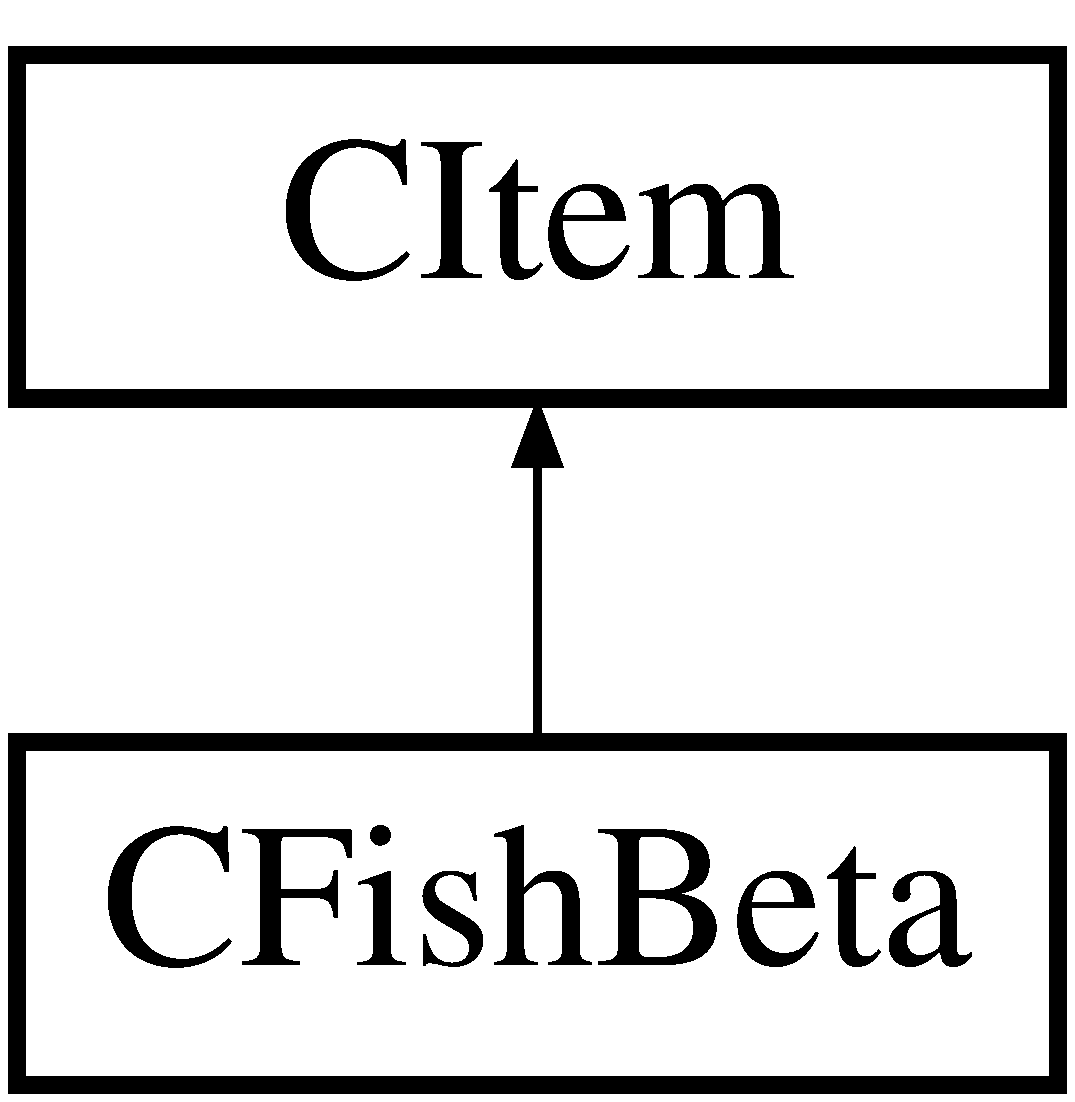
\includegraphics[height=2.000000cm]{class_c_item}
\end{center}
\end{figure}
\subsection*{Public Member Functions}
\begin{DoxyCompactItemize}
\item 
\mbox{\Hypertarget{class_c_item_ac2ea847c008cf8d1de92c870c8f8262f}\label{class_c_item_ac2ea847c008cf8d1de92c870c8f8262f}} 
\mbox{\hyperlink{class_c_item_ac2ea847c008cf8d1de92c870c8f8262f}{C\+Item}} ()=delete
\begin{DoxyCompactList}\small\item\em Default constructor (disabled) \end{DoxyCompactList}\item 
\mbox{\Hypertarget{class_c_item_a7d6042bbb9a571d2dc1d1f89016a97c8}\label{class_c_item_a7d6042bbb9a571d2dc1d1f89016a97c8}} 
\mbox{\hyperlink{class_c_item_a7d6042bbb9a571d2dc1d1f89016a97c8}{C\+Item}} (const \mbox{\hyperlink{class_c_item}{C\+Item}} \&)=delete
\begin{DoxyCompactList}\small\item\em Copy constructor (disabled) \end{DoxyCompactList}\item 
virtual \mbox{\hyperlink{class_c_item_a2487c6e822ed0e850544f1745b43f584}{$\sim$\+C\+Item}} ()
\item 
virtual void \mbox{\hyperlink{class_c_item_a7ef8448d0c4bc53d0f1943a4dc817f6f}{Draw}} (Gdiplus\+::\+Graphics $\ast$graphics)=0
\item 
double \mbox{\hyperlink{class_c_item_a394d38a058fc53f0e958ca52248560c8}{GetX}} () const
\item 
double \mbox{\hyperlink{class_c_item_ac0fe6be80f8ef19854d7f41b4803f658}{GetY}} () const
\item 
void \mbox{\hyperlink{class_c_item_a9c194f3f08e515853600cecca3e6d319}{Set\+Location}} (double x, double y)
\end{DoxyCompactItemize}
\subsection*{Protected Member Functions}
\begin{DoxyCompactItemize}
\item 
\mbox{\hyperlink{class_c_item_a665b3fa4628b43e69b1d7f2b9529882b}{C\+Item}} (\mbox{\hyperlink{class_c_aquarium}{C\+Aquarium}} $\ast$aquarium)
\end{DoxyCompactItemize}


\subsection{Detailed Description}
Instantiation of \mbox{\hyperlink{class_c_item}{C\+Item}} class. Responsible for detecting item movement to pull from. 

\subsection{Constructor \& Destructor Documentation}
\mbox{\Hypertarget{class_c_item_a2487c6e822ed0e850544f1745b43f584}\label{class_c_item_a2487c6e822ed0e850544f1745b43f584}} 
\index{C\+Item@{C\+Item}!````~C\+Item@{$\sim$\+C\+Item}}
\index{````~C\+Item@{$\sim$\+C\+Item}!C\+Item@{C\+Item}}
\subsubsection{\texorpdfstring{$\sim$\+C\+Item()}{~CItem()}}
{\footnotesize\ttfamily C\+Item\+::$\sim$\+C\+Item (\begin{DoxyParamCaption}{ }\end{DoxyParamCaption})\hspace{0.3cm}{\ttfamily [virtual]}}

Destructor \mbox{\Hypertarget{class_c_item_a665b3fa4628b43e69b1d7f2b9529882b}\label{class_c_item_a665b3fa4628b43e69b1d7f2b9529882b}} 
\index{C\+Item@{C\+Item}!C\+Item@{C\+Item}}
\index{C\+Item@{C\+Item}!C\+Item@{C\+Item}}
\subsubsection{\texorpdfstring{C\+Item()}{CItem()}}
{\footnotesize\ttfamily C\+Item\+::\+C\+Item (\begin{DoxyParamCaption}\item[{\mbox{\hyperlink{class_c_aquarium}{C\+Aquarium}} $\ast$}]{aquarium }\end{DoxyParamCaption})\hspace{0.3cm}{\ttfamily [protected]}}

Constructor 
\begin{DoxyParams}{Parameters}
{\em aquarium} & The aquarium that this item is a member of \\
\hline
\end{DoxyParams}


\subsection{Member Function Documentation}
\mbox{\Hypertarget{class_c_item_a7ef8448d0c4bc53d0f1943a4dc817f6f}\label{class_c_item_a7ef8448d0c4bc53d0f1943a4dc817f6f}} 
\index{C\+Item@{C\+Item}!Draw@{Draw}}
\index{Draw@{Draw}!C\+Item@{C\+Item}}
\subsubsection{\texorpdfstring{Draw()}{Draw()}}
{\footnotesize\ttfamily virtual void C\+Item\+::\+Draw (\begin{DoxyParamCaption}\item[{Gdiplus\+::\+Graphics $\ast$}]{graphics }\end{DoxyParamCaption})\hspace{0.3cm}{\ttfamily [pure virtual]}}

Draw this item 
\begin{DoxyParams}{Parameters}
{\em graphics} & Graphics device to draw on \\
\hline
\end{DoxyParams}


Implemented in \mbox{\hyperlink{class_c_fish_beta_ae2effbff7b98bb3cd6e1070d61d5366e}{C\+Fish\+Beta}}.

\mbox{\Hypertarget{class_c_item_a394d38a058fc53f0e958ca52248560c8}\label{class_c_item_a394d38a058fc53f0e958ca52248560c8}} 
\index{C\+Item@{C\+Item}!GetX@{GetX}}
\index{GetX@{GetX}!C\+Item@{C\+Item}}
\subsubsection{\texorpdfstring{Get\+X()}{GetX()}}
{\footnotesize\ttfamily double C\+Item\+::\+GetX (\begin{DoxyParamCaption}{ }\end{DoxyParamCaption}) const\hspace{0.3cm}{\ttfamily [inline]}}

The X location of the item \begin{DoxyReturn}{Returns}
X location in pixels 
\end{DoxyReturn}
\mbox{\Hypertarget{class_c_item_ac0fe6be80f8ef19854d7f41b4803f658}\label{class_c_item_ac0fe6be80f8ef19854d7f41b4803f658}} 
\index{C\+Item@{C\+Item}!GetY@{GetY}}
\index{GetY@{GetY}!C\+Item@{C\+Item}}
\subsubsection{\texorpdfstring{Get\+Y()}{GetY()}}
{\footnotesize\ttfamily double C\+Item\+::\+GetY (\begin{DoxyParamCaption}{ }\end{DoxyParamCaption}) const\hspace{0.3cm}{\ttfamily [inline]}}

The Y location of the item \begin{DoxyReturn}{Returns}
Y location in pixels 
\end{DoxyReturn}
\mbox{\Hypertarget{class_c_item_a9c194f3f08e515853600cecca3e6d319}\label{class_c_item_a9c194f3f08e515853600cecca3e6d319}} 
\index{C\+Item@{C\+Item}!Set\+Location@{Set\+Location}}
\index{Set\+Location@{Set\+Location}!C\+Item@{C\+Item}}
\subsubsection{\texorpdfstring{Set\+Location()}{SetLocation()}}
{\footnotesize\ttfamily void C\+Item\+::\+Set\+Location (\begin{DoxyParamCaption}\item[{double}]{x,  }\item[{double}]{y }\end{DoxyParamCaption})\hspace{0.3cm}{\ttfamily [inline]}}

Set the item location 
\begin{DoxyParams}{Parameters}
{\em x} & X location \\
\hline
{\em y} & Y location \\
\hline
\end{DoxyParams}


The documentation for this class was generated from the following files\+:\begin{DoxyCompactItemize}
\item 
\mbox{\hyperlink{_item_8h}{Item.\+h}}\item 
\mbox{\hyperlink{_item_8cpp}{Item.\+cpp}}\end{DoxyCompactItemize}

\hypertarget{class_c_main_frame}{}\section{C\+Main\+Frame Class Reference}
\label{class_c_main_frame}\index{C\+Main\+Frame@{C\+Main\+Frame}}
Inheritance diagram for C\+Main\+Frame\+:\begin{figure}[H]
\begin{center}
\leavevmode
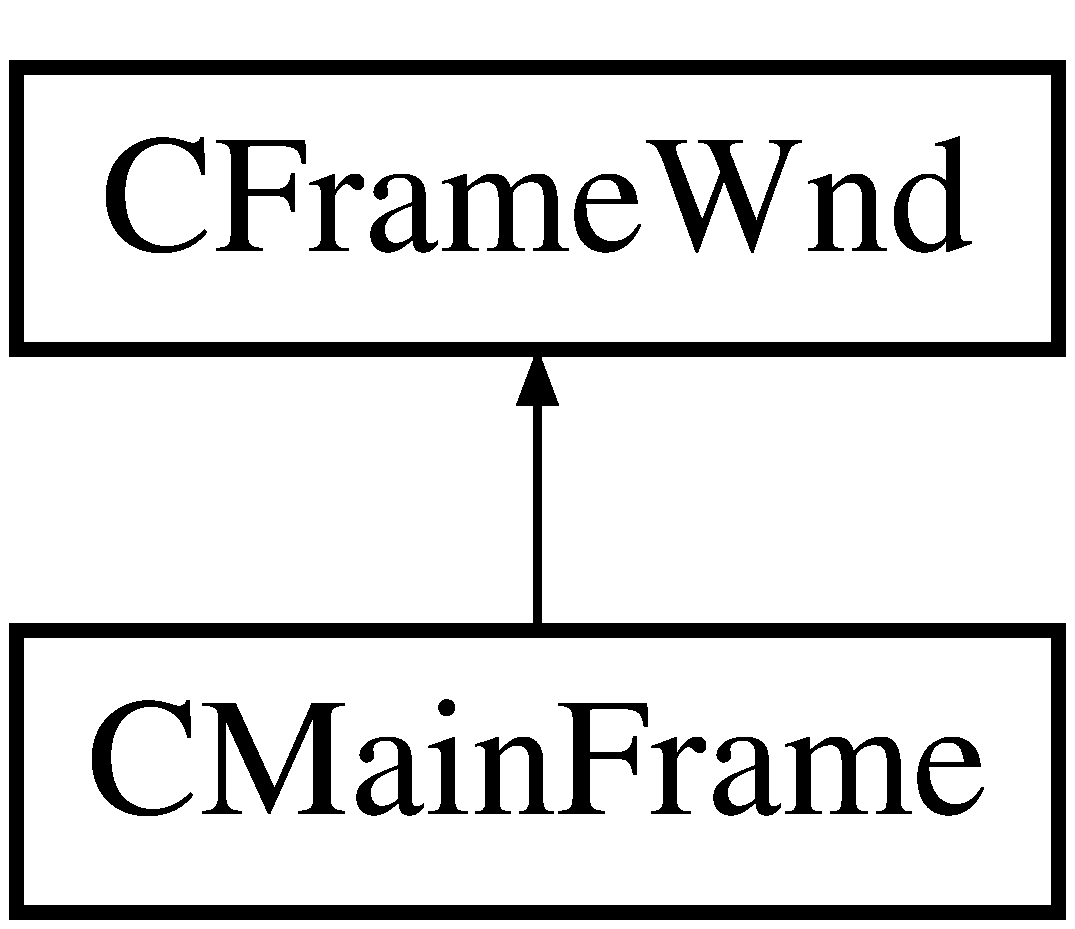
\includegraphics[height=2.000000cm]{class_c_main_frame}
\end{center}
\end{figure}
\subsection*{Public Member Functions}
\begin{DoxyCompactItemize}
\item 
virtual B\+O\+OL \mbox{\hyperlink{class_c_main_frame_a549bf677c955c2898c3c683321633c16}{Pre\+Create\+Window}} (C\+R\+E\+A\+T\+E\+S\+T\+R\+U\+CT \&cs)
\item 
virtual B\+O\+OL \mbox{\hyperlink{class_c_main_frame_ade959eb0bab719bf06bb9b18ee407101}{On\+Cmd\+Msg}} (U\+I\+NT n\+ID, int n\+Code, void $\ast$p\+Extra, A\+F\+X\+\_\+\+C\+M\+D\+H\+A\+N\+D\+L\+E\+R\+I\+N\+FO $\ast$p\+Handler\+Info)
\end{DoxyCompactItemize}
\subsection*{Protected Member Functions}
\begin{DoxyCompactItemize}
\item 
afx\+\_\+msg int \mbox{\hyperlink{class_c_main_frame_a48666466fd37412fcaeff75c3b12e0ed}{On\+Create}} (L\+P\+C\+R\+E\+A\+T\+E\+S\+T\+R\+U\+CT lp\+Create\+Struct)
\item 
afx\+\_\+msg void \mbox{\hyperlink{class_c_main_frame_adc353a3d1fc497fbc009b6d9e6914a82}{On\+Set\+Focus}} (C\+Wnd $\ast$p\+Old\+Wnd)
\end{DoxyCompactItemize}
\subsection*{Protected Attributes}
\begin{DoxyCompactItemize}
\item 
\mbox{\Hypertarget{class_c_main_frame_a73024d794dce2fe918f6b117371c25fc}\label{class_c_main_frame_a73024d794dce2fe918f6b117371c25fc}} 
C\+Tool\+Bar {\bfseries m\+\_\+wnd\+Tool\+Bar}
\item 
\mbox{\Hypertarget{class_c_main_frame_ac01bafc03aee69cf982e6f029b4db6b0}\label{class_c_main_frame_ac01bafc03aee69cf982e6f029b4db6b0}} 
C\+Status\+Bar {\bfseries m\+\_\+wnd\+Status\+Bar}
\item 
\mbox{\Hypertarget{class_c_main_frame_a7c3af9327c496f8c807d578f7a4ef4c5}\label{class_c_main_frame_a7c3af9327c496f8c807d578f7a4ef4c5}} 
\mbox{\hyperlink{class_c_child_view}{C\+Child\+View}} {\bfseries m\+\_\+wnd\+View}
\end{DoxyCompactItemize}


\subsection{Member Function Documentation}
\mbox{\Hypertarget{class_c_main_frame_ade959eb0bab719bf06bb9b18ee407101}\label{class_c_main_frame_ade959eb0bab719bf06bb9b18ee407101}} 
\index{C\+Main\+Frame@{C\+Main\+Frame}!On\+Cmd\+Msg@{On\+Cmd\+Msg}}
\index{On\+Cmd\+Msg@{On\+Cmd\+Msg}!C\+Main\+Frame@{C\+Main\+Frame}}
\subsubsection{\texorpdfstring{On\+Cmd\+Msg()}{OnCmdMsg()}}
{\footnotesize\ttfamily B\+O\+OL C\+Main\+Frame\+::\+On\+Cmd\+Msg (\begin{DoxyParamCaption}\item[{U\+I\+NT}]{n\+ID,  }\item[{int}]{n\+Code,  }\item[{void $\ast$}]{p\+Extra,  }\item[{A\+F\+X\+\_\+\+C\+M\+D\+H\+A\+N\+D\+L\+E\+R\+I\+N\+FO $\ast$}]{p\+Handler\+Info }\end{DoxyParamCaption})\hspace{0.3cm}{\ttfamily [virtual]}}

Checking for command messages 
\begin{DoxyParams}{Parameters}
{\em n\+ID} & \\
\hline
{\em n\+Code} & \\
\hline
{\em p\+Extra} & \\
\hline
{\em p\+Handler\+Info} & \\
\hline
\end{DoxyParams}
\begin{DoxyReturn}{Returns}

\end{DoxyReturn}
\mbox{\Hypertarget{class_c_main_frame_a48666466fd37412fcaeff75c3b12e0ed}\label{class_c_main_frame_a48666466fd37412fcaeff75c3b12e0ed}} 
\index{C\+Main\+Frame@{C\+Main\+Frame}!On\+Create@{On\+Create}}
\index{On\+Create@{On\+Create}!C\+Main\+Frame@{C\+Main\+Frame}}
\subsubsection{\texorpdfstring{On\+Create()}{OnCreate()}}
{\footnotesize\ttfamily int C\+Main\+Frame\+::\+On\+Create (\begin{DoxyParamCaption}\item[{L\+P\+C\+R\+E\+A\+T\+E\+S\+T\+R\+U\+CT}]{lp\+Create\+Struct }\end{DoxyParamCaption})\hspace{0.3cm}{\ttfamily [protected]}}

Creation of Mainframe window 
\begin{DoxyParams}{Parameters}
{\em lp\+Create\+Struct} & \\
\hline
\end{DoxyParams}
\begin{DoxyReturn}{Returns}

\end{DoxyReturn}
\mbox{\Hypertarget{class_c_main_frame_adc353a3d1fc497fbc009b6d9e6914a82}\label{class_c_main_frame_adc353a3d1fc497fbc009b6d9e6914a82}} 
\index{C\+Main\+Frame@{C\+Main\+Frame}!On\+Set\+Focus@{On\+Set\+Focus}}
\index{On\+Set\+Focus@{On\+Set\+Focus}!C\+Main\+Frame@{C\+Main\+Frame}}
\subsubsection{\texorpdfstring{On\+Set\+Focus()}{OnSetFocus()}}
{\footnotesize\ttfamily void C\+Main\+Frame\+::\+On\+Set\+Focus (\begin{DoxyParamCaption}\item[{C\+Wnd $\ast$}]{p\+Old\+Wnd }\end{DoxyParamCaption})\hspace{0.3cm}{\ttfamily [protected]}}

Setting the focus of the mainframe window \mbox{\hyperlink{class_c_main_frame}{C\+Main\+Frame}} message handlers 
\begin{DoxyParams}{Parameters}
{\em } & \\
\hline
\end{DoxyParams}
\mbox{\Hypertarget{class_c_main_frame_a549bf677c955c2898c3c683321633c16}\label{class_c_main_frame_a549bf677c955c2898c3c683321633c16}} 
\index{C\+Main\+Frame@{C\+Main\+Frame}!Pre\+Create\+Window@{Pre\+Create\+Window}}
\index{Pre\+Create\+Window@{Pre\+Create\+Window}!C\+Main\+Frame@{C\+Main\+Frame}}
\subsubsection{\texorpdfstring{Pre\+Create\+Window()}{PreCreateWindow()}}
{\footnotesize\ttfamily B\+O\+OL C\+Main\+Frame\+::\+Pre\+Create\+Window (\begin{DoxyParamCaption}\item[{C\+R\+E\+A\+T\+E\+S\+T\+R\+U\+CT \&}]{cs }\end{DoxyParamCaption})\hspace{0.3cm}{\ttfamily [virtual]}}

Pre\+Creation of Main\+Frame Window for Aquarium 
\begin{DoxyParams}{Parameters}
{\em cs} & \\
\hline
\end{DoxyParams}
\begin{DoxyReturn}{Returns}

\end{DoxyReturn}


The documentation for this class was generated from the following files\+:\begin{DoxyCompactItemize}
\item 
Main\+Frm.\+h\item 
Main\+Frm.\+cpp\end{DoxyCompactItemize}

\hypertarget{class_c_step2_app}{}\section{C\+Step2\+App Class Reference}
\label{class_c_step2_app}\index{C\+Step2\+App@{C\+Step2\+App}}
Inheritance diagram for C\+Step2\+App\+:\begin{figure}[H]
\begin{center}
\leavevmode
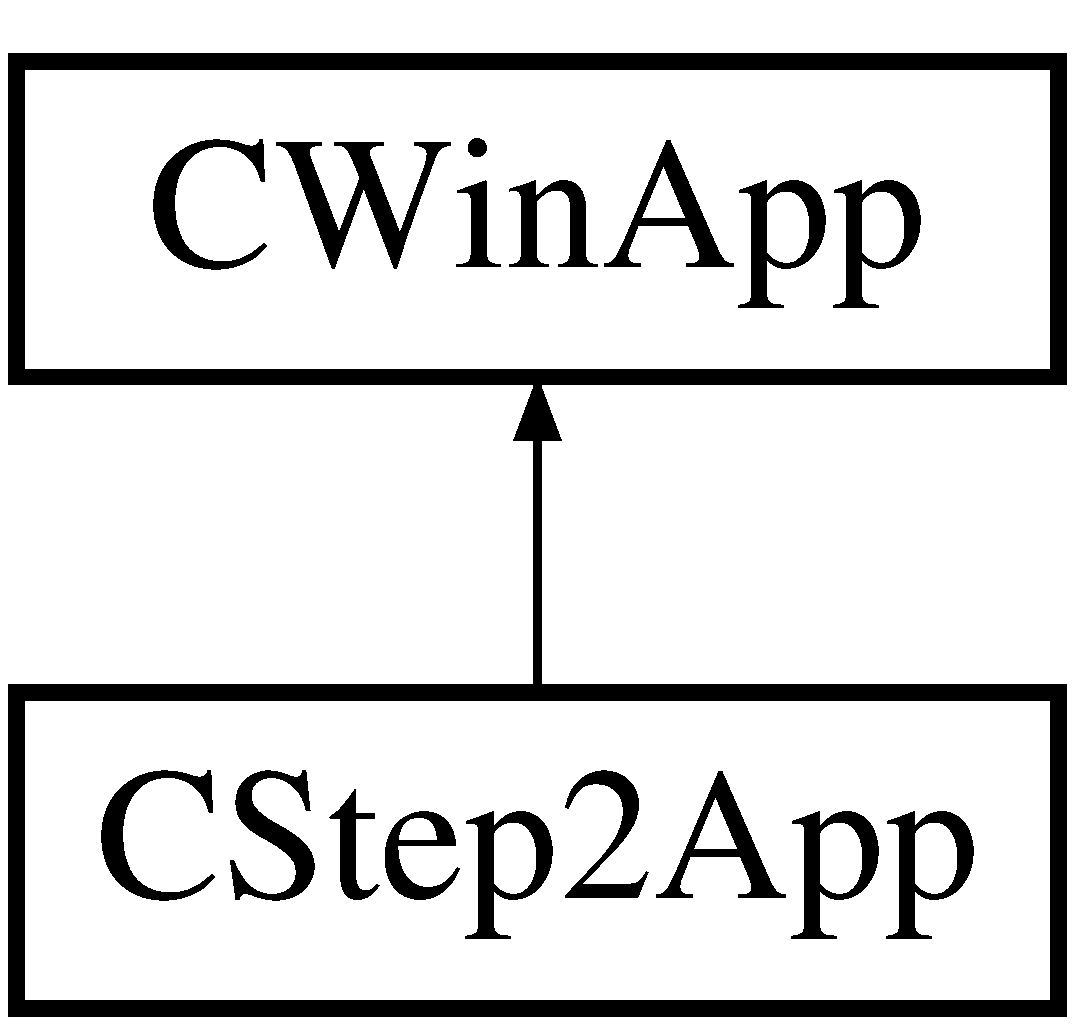
\includegraphics[height=2.000000cm]{class_c_step2_app}
\end{center}
\end{figure}
\subsection*{Public Member Functions}
\begin{DoxyCompactItemize}
\item 
\mbox{\Hypertarget{class_c_step2_app_a4152bf861e6e520eaa173c41a3d9f73d}\label{class_c_step2_app_a4152bf861e6e520eaa173c41a3d9f73d}} 
virtual B\+O\+OL {\bfseries Init\+Instance} ()
\item 
\mbox{\Hypertarget{class_c_step2_app_aad455705e63bb9ae0642be6ca2d2b684}\label{class_c_step2_app_aad455705e63bb9ae0642be6ca2d2b684}} 
virtual int {\bfseries Exit\+Instance} ()
\item 
\mbox{\Hypertarget{class_c_step2_app_a7407f02b1d0628458512c9f35ab2bb50}\label{class_c_step2_app_a7407f02b1d0628458512c9f35ab2bb50}} 
afx\+\_\+msg void {\bfseries On\+App\+About} ()
\end{DoxyCompactItemize}


The documentation for this class was generated from the following files\+:\begin{DoxyCompactItemize}
\item 
Step2.\+h\item 
Step2.\+cpp\end{DoxyCompactItemize}

\chapter{File Documentation}
\hypertarget{_aquarium_8cpp}{}\section{Aquarium.\+cpp File Reference}
\label{_aquarium_8cpp}\index{Aquarium.\+cpp@{Aquarium.\+cpp}}
{\ttfamily \#include \char`\"{}stdafx.\+h\char`\"{}}\newline
{\ttfamily \#include \char`\"{}Aquarium.\+h\char`\"{}}\newline
{\ttfamily \#include $<$memory$>$}\newline


\subsection{Detailed Description}
\begin{DoxyAuthor}{Author}
Mark Maroki 
\end{DoxyAuthor}

\hypertarget{_aquarium_8h}{}\section{Aquarium.\+h File Reference}
\label{_aquarium_8h}\index{Aquarium.\+h@{Aquarium.\+h}}
{\ttfamily \#include $<$memory$>$}\newline
\subsection*{Classes}
\begin{DoxyCompactItemize}
\item 
class \mbox{\hyperlink{class_c_aquarium}{C\+Aquarium}}
\end{DoxyCompactItemize}


\subsection{Detailed Description}
\begin{DoxyAuthor}{Author}
Mark Maroki Class that implements the Aquarium window. 
\end{DoxyAuthor}

\hypertarget{_child_view_8cpp}{}\section{Child\+View.\+cpp File Reference}
\label{_child_view_8cpp}\index{Child\+View.\+cpp@{Child\+View.\+cpp}}
{\ttfamily \#include \char`\"{}stdafx.\+h\char`\"{}}\newline
{\ttfamily \#include \char`\"{}Step2.\+h\char`\"{}}\newline
{\ttfamily \#include \char`\"{}Child\+View.\+h\char`\"{}}\newline


\subsection{Detailed Description}
\begin{DoxyAuthor}{Author}
Mark Maroki 
\end{DoxyAuthor}

\hypertarget{_child_view_8h}{}\section{Child\+View.\+h File Reference}
\label{_child_view_8h}\index{Child\+View.\+h@{Child\+View.\+h}}
{\ttfamily \#include \char`\"{}Aquarium.\+h\char`\"{}}\newline
\subsection*{Classes}
\begin{DoxyCompactItemize}
\item 
class \mbox{\hyperlink{class_c_child_view}{C\+Child\+View}}
\end{DoxyCompactItemize}


\subsection{Detailed Description}
\begin{DoxyAuthor}{Author}
Mark Maroki
\end{DoxyAuthor}
Class that implements child window the program draws in.

The window is a child of the main frame, which holds the window, the menu bar, and the status bar. 
\hypertarget{_fish_beta_8cpp}{}\section{Fish\+Beta.\+cpp File Reference}
\label{_fish_beta_8cpp}\index{Fish\+Beta.\+cpp@{Fish\+Beta.\+cpp}}
{\ttfamily \#include \char`\"{}stdafx.\+h\char`\"{}}\newline
{\ttfamily \#include \char`\"{}Fish\+Beta.\+h\char`\"{}}\newline


\subsection{Detailed Description}
\begin{DoxyAuthor}{Author}
Mark Maroki 
\end{DoxyAuthor}

\hypertarget{_fish_beta_8h}{}\section{Fish\+Beta.\+h File Reference}
\label{_fish_beta_8h}\index{Fish\+Beta.\+h@{Fish\+Beta.\+h}}
{\ttfamily \#include \char`\"{}Item.\+h\char`\"{}}\newline
\subsection*{Classes}
\begin{DoxyCompactItemize}
\item 
class \mbox{\hyperlink{class_c_fish_beta}{C\+Fish\+Beta}}
\end{DoxyCompactItemize}


\subsection{Detailed Description}
\begin{DoxyAuthor}{Author}
Mark Maroki Beta Fish class derived from Items class. 
\end{DoxyAuthor}

\hypertarget{_item_8cpp}{}\section{Item.\+cpp File Reference}
\label{_item_8cpp}\index{Item.\+cpp@{Item.\+cpp}}
{\ttfamily \#include \char`\"{}stdafx.\+h\char`\"{}}\newline
{\ttfamily \#include \char`\"{}Item.\+h\char`\"{}}\newline
{\ttfamily \#include \char`\"{}Aquarium.\+h\char`\"{}}\newline


\subsection{Detailed Description}
\begin{DoxyAuthor}{Author}
Mark Maroki 
\end{DoxyAuthor}

\hypertarget{_item_8h}{}\section{Item.\+h File Reference}
\label{_item_8h}\index{Item.\+h@{Item.\+h}}
\subsection*{Classes}
\begin{DoxyCompactItemize}
\item 
class \mbox{\hyperlink{class_c_item}{C\+Item}}
\end{DoxyCompactItemize}


\subsection{Detailed Description}
Item Class is used to track the Items in the Aquarium. Therefore is a child? \begin{DoxyAuthor}{Author}
Mark Maroki 
\end{DoxyAuthor}

%--- End generated contents ---

% Index
\backmatter
\newpage
\phantomsection
\clearemptydoublepage
\addcontentsline{toc}{chapter}{Index}
\printindex

\end{document}
